% \documentclass[a4paper,11pt]{article}
% \usepackage[hyperref]{beamerarticle}

\documentclass[final]{beamer}

\usepackage[hangul]{kotex}
\usepackage{amsfonts,amsmath,xob-amssymb}

\usepackage{amsthm}
\newtheorem{defn}{Definition}
\newtheorem{thm}{Theorem}

\usepackage{cancel}
\graphicspath{{./_img/04/}}

\usepackage{graphicx}
\usepackage{media9}
\usepackage{tikz}
\usepackage{textpos}

\mode<presentation>{
	\usetheme{Madrid}
	\usecolortheme{default}
	\usefonttheme{professionalfonts}
}

\def\b{\boldsymbol}

\mode<article>{
\usepackage{fullpage}
}
\usepackage{ulem}

\newcommand{\bb}{\mathbb}
\newcommand{\bd}{\mathbf}
\newcommand{\p}{\partial}

\newcounter{saveenumi}
\newcommand{\seti}{\setcounter{saveenumi}{\value{enumi}}}
\newcommand{\conti}{\setcounter{enumi}{\value{saveenumi}}}

\newcommand{\mail}{\url{mailto:experiment.namun+2016f@gmail.com} }


\title{게임이론 Part 2}
\subtitle{게임의 기본 개념들 (게임이론, 진화, 그리고 협력)}
\author[조남운]{허준석$\rightarrow$이동한$\rightarrow$\emph{조남운}\\\mail}

\begin{document}

\begin{frame}[t]{}
	\titlepage
\end{frame}
%--- Next Frame ---%

\begin{frame}[t]{목차}
	\tableofcontents
\end{frame}
%--- Next Frame ---%

\section{전략형 게임(Strategic Form Game)} % (fold)
\label{sec:StrategicForm}

\begin{frame}[t]{조정 게임의 변형: 성대결 게임 (Battle of Sexes)}
	\begin{columns}
		\column{.6\textwidth}
		\begin{itemize}
			% \item 이해관계는 같음
			\item 두 개의 균형
			\item 어떤 균형이냐에 따라 이득이 달라짐
			\item 실제 사례가 존재할까?
		\end{itemize}
		\column{.4\textwidth}
		\begin{center}
			\begin{table}
				\setlength{\tabcolsep}{1.2em}
				\begin{tabular}{|c|c|c|} \hline
				& {F} &  {B} \\ \hline
				{F} & {$2$}, {$1$} & {$0$}, {$0$} \\ \hline%
				{B} & {$0$}, {$0$}  & {$1$}, {$2$} \\ 
				\hline
				\end{tabular}
			\end{table}
		\end{center}
	\end{columns}
\end{frame}
%--- Next Frame ---%

\begin{frame}[t]{조정 게임의 변형(2): Stag Hunt Game}
	\begin{columns}[c]
	\column{13em}
	\begin{itemize}
		\item J.J. 루소가 고안  
		\item 옆의 그림을 보자 
		\item 어떤 사례에 해당할까? 
	\end{itemize}
	\column{16em}
	\hspace{-1em}
	\begin{center}
	\fbox{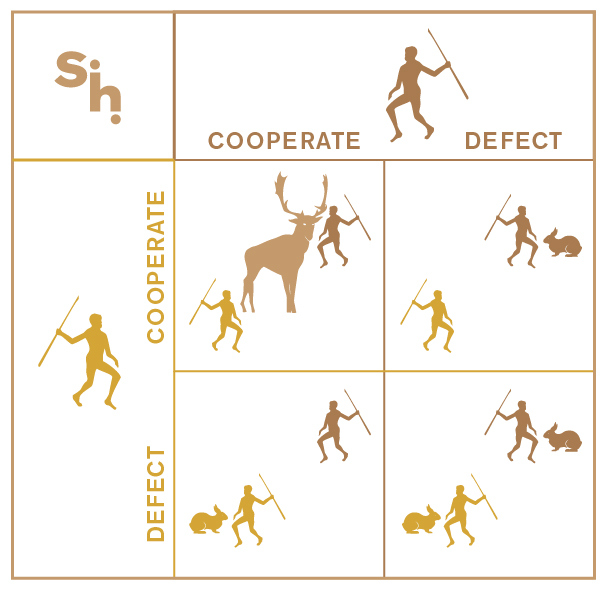
\includegraphics[width=10em]{staghunt.jpg}}
	\begin{table}
	\setlength{\tabcolsep}{1.2em}
	\begin{tabular}{|c|c|c|} \hline
	& {S} &  {H} \\ \hline
	{S} & {$3$}, {$3$} & {$0$}, {$2$} \\ \hline%
	{H} & {$2$}, {$0$}  & {$1$}, {$1$} \\ 
	\hline
	\end{tabular}
	\end{table}
	\end{center}
	\end{columns}
\end{frame}
%--- Next Frame ---%

\begin{frame}[t]{조정게임에서 MSNE 찾기}
	\begin{itemize}
		\item 앞서 존 내시의 공헌은 균형이 존재한다는 것을 증명한 것
		\item 앞서의 게임에서도 MSNE을 찾을 수 있을까?
		\item Mission:
			\begin{enumerate}
			\item MSNE(혼합전략 내쉬균형)을 찾아라!
			\item PSNE(순수전략 내쉬균형)과 MSNE에서의 payoff를 비교하라!	
			\end{enumerate}
		\item Correlated equilibrium	
	\end{itemize}
\end{frame}
%--- Next Frame ---%

\begin{frame}[t]{Volunteer Dilemma I}
	\begin{columns}[c]
	\column{18em}
	\begin{itemize}
		\item 집 밖에서 들려오는 다급한 도와달라는 비명소리 
		\item 누군가 전화를 걸면 그는 무사, 하지만 아무도 걸지 않으면 죽을 수도 있다. 
		\item 이 타인이 죽는다면 동네 사람들의 보수는 0, 무사하면 1
		\item 전화를 거는 비용은 $0<c<1$
	\end{itemize}
	\column{15em}\hspace{0em}
	\fbox{
\includegraphics[width=12em]{ecall.jpg}}
	\end{columns}
\end{frame}
%--- Next Frame ---%

\begin{frame}[t]{Volunteer Dilemma II}
	\begin{columns}[c]
	\column{18em}
	\begin{itemize}
		\item 2명만 있다고 보고 보수 행렬 만들기
		\item 어떤 게임인가? 
		\item PSNE과  MSNE을 각각 구해보라. 
		\item 2명이 아니라 $n(>2)$ 명이라면?
	    \item 역시 PSNE와 MSNE를 구해보라. 
	\end{itemize}
	\column{13em}
	\begin{align*}
	&\overbrace{1-c}^{\text{다른 1명이 전화를 걸 때 보수}} \\
	&= \\
	&\hspace{-1em}\underbrace{1 \times [1-(1-p)^{n-1}].}_{\text{다른 1명이 전화를 걸지 않을 때 보수}}
	\end{align*}
	따라서, MSNE이 되는 $p^*$는 
	\[ p^* = 1-c^{\frac{1}{n-1}}  \]
	$n$이 증가할수록 $p^*$는? 
	\end{columns}
\end{frame}
%--- Next Frame ---%

% section StrategicForm (end)


\section{전개형 게임(Extensive Form Game)} % (fold)
\label{sec:extensiveForm}

\begin{frame}[t]{전개형 게임}
	\begin{itemize}
		\item 지금까지 살펴본 게임방식:
		\begin{itemize}
			\item 플레이어는 상대방의 결정을 모른채 전략적 결정을 내린다
			\item 게임은 1회만 진행한다
		\end{itemize}
		\item 위 두 방식의 변형
		\begin{itemize}
			\item 상대의 결정을 안다: 전개형 게임
			\item 상대와 여러번 게임을 한다: 반복 게임
		\end{itemize}
	\end{itemize}
\end{frame}
%--- Next Frame ---%

\begin{frame}[t]{전개형 게임의 요소}
	\begin{itemize}
		\item 선수들
		\item 액션들과 전략
		\item \uline{선택 노드들과 가지}: Game Tree
		\item 정보 집합 (무엇을 알고 무엇을 모르는지에 대한 규정)
	\end{itemize}
\end{frame}
%--- Next Frame ---%

\begin{frame}[t]{Game Tree}
	\begin{center}
	\fbox{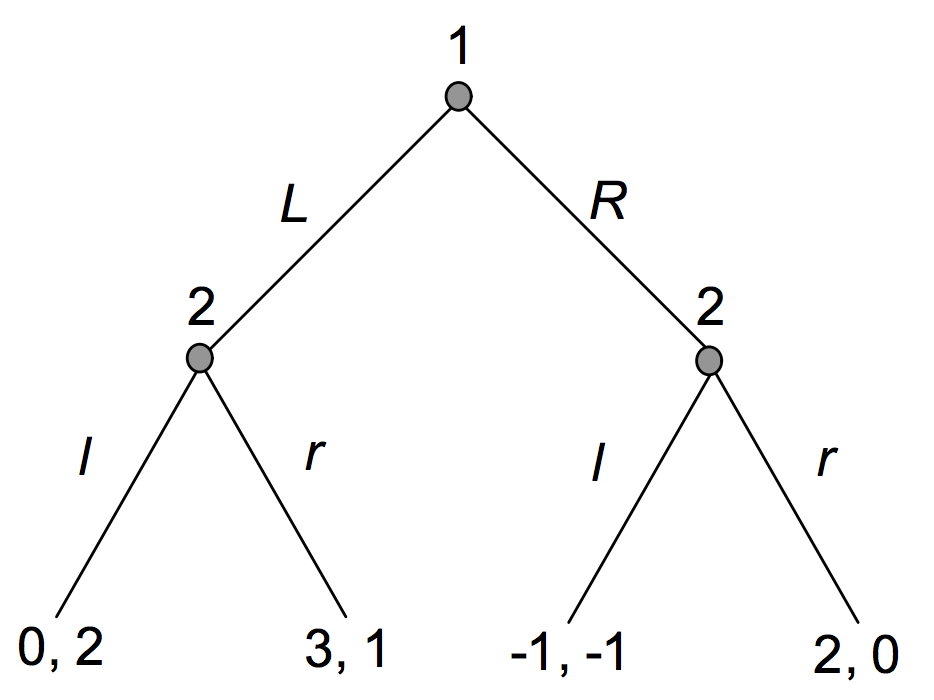
\includegraphics[width=22em]{tree_1.png}}
	\end{center}
\end{frame}
%--- Next Frame ---%

\begin{frame}[t]{전개형 게임에서 균형찾기}
	\begin{columns}[c]
	\column{15em}
	\begin{itemize}
		\item 우리는 전략과 행동의 차이에 대해서 이미 배웠다. 
		\item $P1$의 전략은? $P2$의 전략은?
	\end{itemize}
	\column{15em}
	\begin{itemize}
		\item 연습문제 
		\begin{enumerate}
			\item 앞서의 전개형 게임을 전략형 게임의 보수행렬로 나타내보라.
			\item 내시 균형을 찾아보라. 
		\end{enumerate}
	\end{itemize}
	\end{columns}
\end{frame}
%--- Next Frame ---%

\begin{frame}\frametitle{이 균형은 만족스러운가?}\vspace{3em}
%\begin{columns}[c]
%\column{13em}
\begin{itemize}
	\item 이상하다고 느껴지는 균형이 있는가? 
	\item 만일 이상하다면 왜 이상한가? 
	\item 균형을 찾기 위해 전개형 게임을 전랴형으로 축약하는 과정에서 잃은 것은 없는가? 
\end{itemize}
%\column{15em}
%\end{columns}
\end{frame}

\begin{frame}[t]{Equilibrium Refinement}
	\begin{columns}[c]
	\column{20em}
	\begin{itemize}
		\item 균형이 너무 많으면 균형으로서 힘을 잃는다. 
		\item 여러 개의 균형 중에서 보다 의미 있는 것과 아닌 것을 구별할 수 있는 방법은?
		\item 이제 전개형 게임에서 최초의 균형 선택 과정이 나타나게 된다. 
	\end{itemize}
	\column{13em}
	\fbox{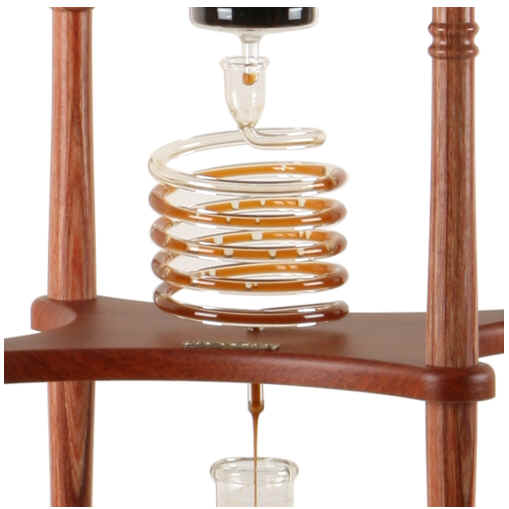
\includegraphics[width=12em]{refinement.jpg}}
	\end{columns}
\end{frame}
%--- Next Frame ---%

\begin{frame}[t]{역지사지}
	\begin{columns}[c]
	\column{18em}
	\begin{itemize}
		\item 상대의 입장에서 먼저 생각한다. 
		\item 전개형 게임에서는 누가 이렇게 생각해야 하나? 
	\end{itemize}
	\column{15em}\hspace{-2em}
	\fbox{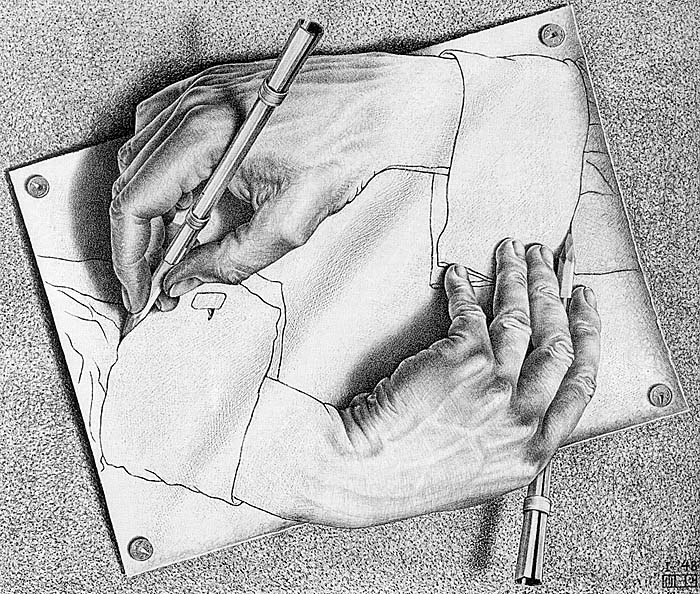
\includegraphics[width=14em]{EsherHand.jpg}}
	\end{columns}
\end{frame}
%--- Next Frame ---%

\begin{frame}[t]{Subgame}
	\begin{columns}[c]
	\column{20em}
	\begin{itemize}
		\item 전개형 게임에서 원래 게임에서 떼어낼 수 있는 부분
		\item 이렇게 떼어낸 후 무엇이 좋은지 생각한다. 
		\item 서브게임은 어디에서부터 생겨나는가? 
		\item 역진귀납법, 후방추론법 \\(backward induction)
	\end{itemize}
	\column{15em}
	\fbox{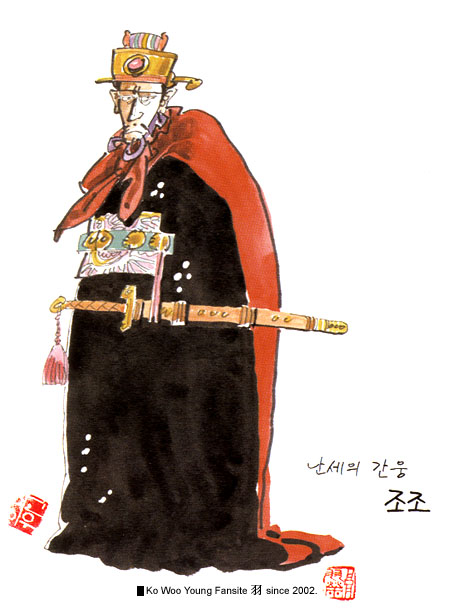
\includegraphics[width=13em]{jojo.jpg}}
	\end{columns}
\end{frame}
%--- Next Frame ---%

\begin{frame}\frametitle{Sub-game Perfect Equilibrium}\vspace{3em}
%\begin{columns}[c]
%\column{20em}
\begin{itemize}
	\item 이렇게 모든 원래 게임 및 그 서브게임들에서 최적화 선택을 완전히 적용할 때 
	\item 이런 균형 상태를 SPE이라고 한다. 
	\item SPE $\subseteq$ NE?
\end{itemize}
%\column{15em}
%\fbox{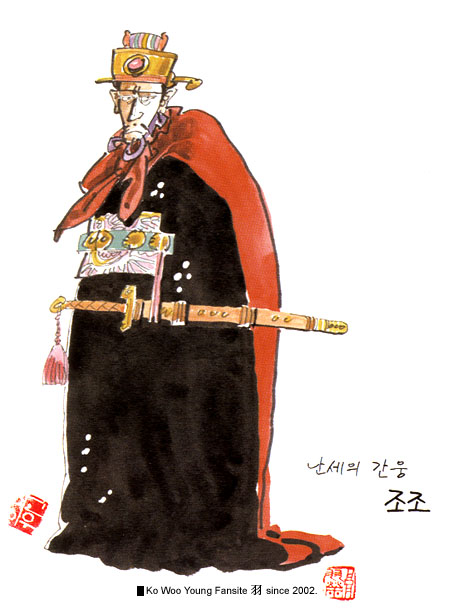
\includegraphics[width=13em]{jojo.jpg}}
%\end{columns}
\end{frame}

\begin{frame}[t]{Chain Store Game}
	\begin{columns}[c]
	\column{.5\textwidth}
	\begin{itemize}
		\item 옆의 게임에 SPE를 찾아보자.
		\item 당신이 $P2$(Chain Store)이라면 어떻게 하겠는가?
	\end{itemize}
	\column{.5\textwidth}
	\fbox{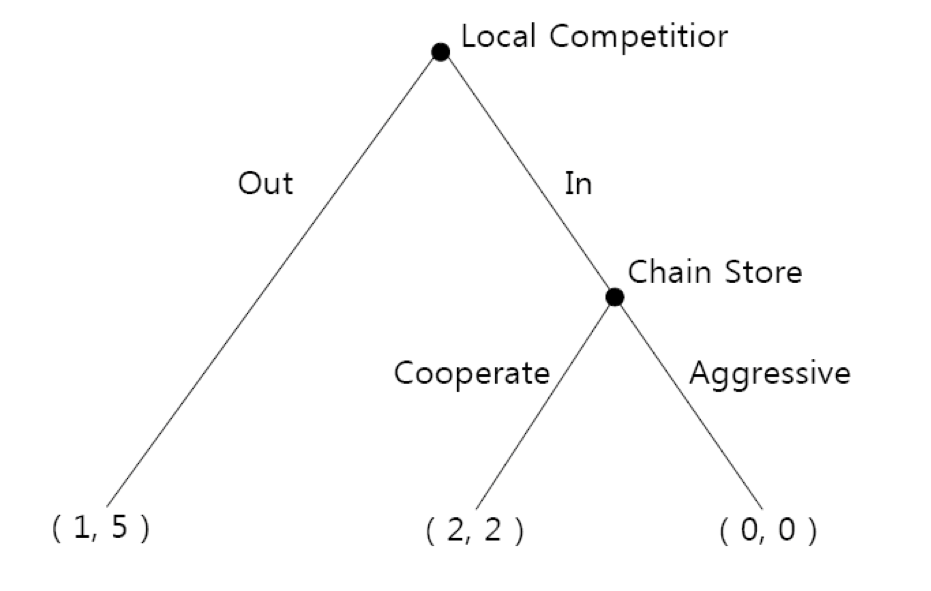
\includegraphics[width=\textwidth]{chainstore01.png}}
	\end{columns}
\end{frame}
%--- Next Frame ---%

\begin{frame}[t]{Credible Threat/Commitment}
	\begin{columns}[c]
	\column{20em}
	\begin{itemize}
		\item 게임이 시작하기 전에, 
		``나는 네가 들어오는 순간 무조건 $l$이야!''
		\item 하지만 게임이론의 입장에서 이러한 협박은 설득력이 있을까? 
	\end{itemize}
	\column{13em} 
	\fbox{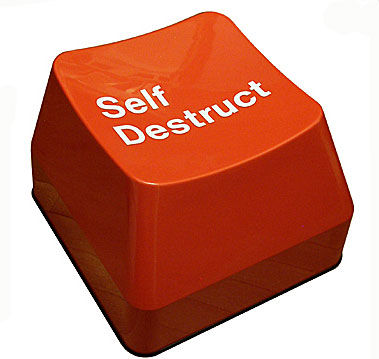
\includegraphics[width=12em]{ct.jpg}}
	\end{columns}
\end{frame}
%--- Next Frame ---%

\begin{frame}[t]{어떻게 믿을 수 있게 만드는가}
	\begin{columns}[c]
	\column{20em}
	\begin{itemize}
		\item 일단 저 선택에 들어서면 이미 늦는다. 
		\item 희생없는 협박은 상대에게 위협이 되지 않는다. 
		\begin{enumerate}
			\item 정치인들의 공약 및 선언
			\item 미리 상당한 비용을 지불해버리기
			\item 배수의 진
		\end{enumerate}
	\end{itemize}
	\column{13em} 
	\fbox{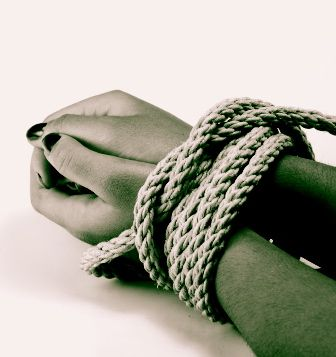
\includegraphics[width=12em]{handtie.jpg}}
	\end{columns}
\end{frame}
%--- Next Frame ---%

\begin{frame}[t]{Paradox of Backward Induction I}
	%\begin{columns}[c]
	%\column{20em}
	\begin{center}
	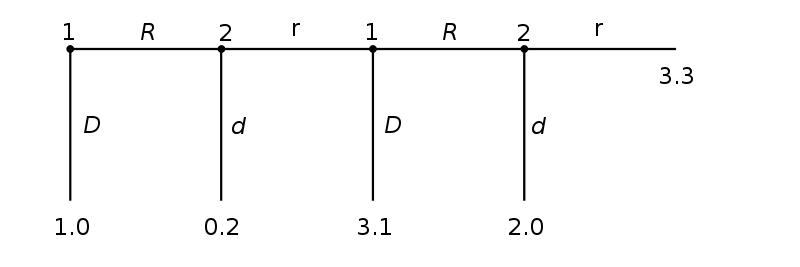
\includegraphics[width=33em]{centepede.png}
	\end{center}
	\begin{itemize}
		\item 역진귀납에 따르면 이 게임의 균형은?
		\item 하지만 이러한 균형은 `합리적'인가? 
	\end{itemize}
	%\column{13em} 
	%\fbox{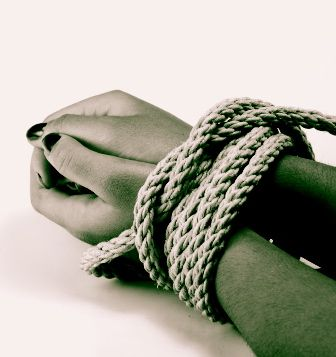
\includegraphics[width=12em]{handtie.jpg}}
	%\end{columns}
\end{frame}
%--- Next Frame ---%

\begin{frame}[t]{Paradox of Backward Induction II}
	\begin{columns}[c]
	\column{15em}
	\begin{itemize}
		\item 축약된 최후통첩 게임
		\item 역진귀납에 따른 균형은? 
		\item 하지만 이 균형은 당신의 `감성'에 호소하는가?
	\end{itemize}
	\column{15em} 
	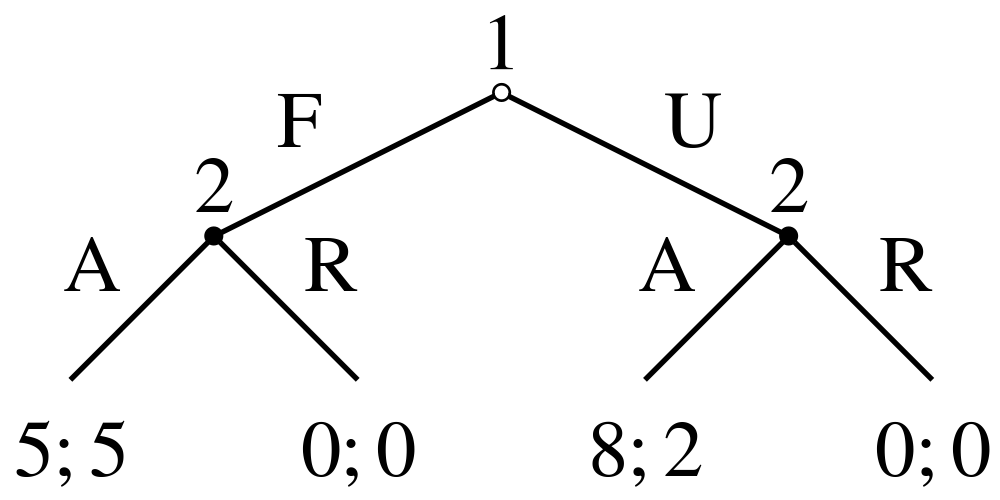
\includegraphics[width=13em]{Ultimatum_Game_Extensive_Form.png}
	\end{columns}
\end{frame}
%--- Next Frame ---%

\begin{frame}[t]{Ultimatum Game}
	\begin{center}
	\fbox{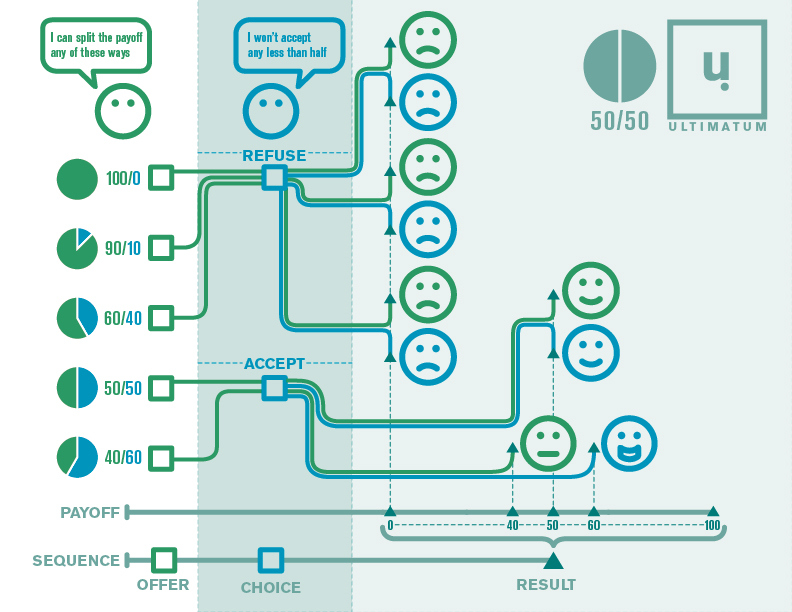
\includegraphics[width=.7\textwidth]{ultimatum.jpg}}
	\end{center}
\end{frame}
%--- Next Frame ---%

\begin{frame}[t]{Understanding Ultimatum Game}
	\begin{columns}[c]
	\column{15em}
	\begin{itemize}
		\item rationality의 부족 
		\item 금전적인 손해, 하지만 심리적인 보상 
		\item Inequality aversion 
		\item 뇌의 화학 작용의 일부로 이해 
	\end{itemize}
	\column{15em} 
	\fbox{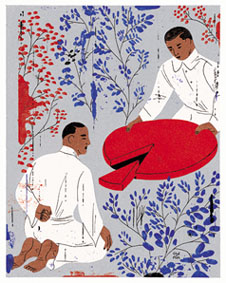
\includegraphics[width=13em]{ult.jpg}}
	\end{columns}
\end{frame}
%--- Next Frame ---%

\begin{frame}\frametitle{Pirate Game}\vspace{0em}
\begin{columns}[c]
\column{19em}
\begin{itemize}
	\item 5인의 해적 ( $A>B>C>D>E$ )
	\item 100만큼의 보석을 발견 
	\item 연장자 순으로 몫 제안
	\item 찬반 투표로 동율 이상이면 채택 
	\item  부결되면 제안자는 바다에 뎐져지고 다음 연장자가 다시 제안
	\begin{enumerate}
		\item 일단 생존이 중요 (죽으면 소용 없음) 
		\item 많은 몫을 챙기고자 하며 
		\item 서로를 믿지 않아서 여러 형태의 담합은 불가 
	\end{enumerate}
\end{itemize}
\column{15em} 
\fbox{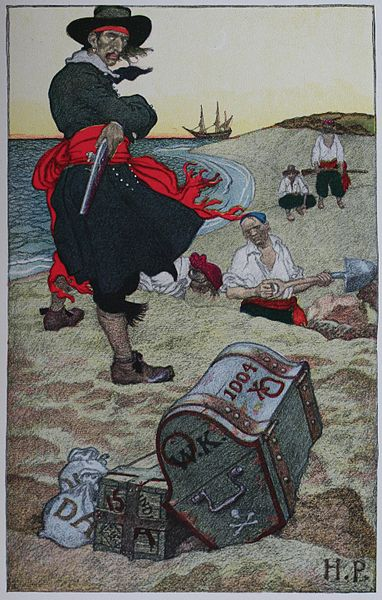
\includegraphics[width=13em]{pirate.jpg}}
\end{columns}
\end{frame}

\begin{frame}[t]{Blotto Game}
	\begin{columns}[c]
	\column{19em}
	\begin{itemize}
		\item n(>5)의 자원을 양측이 가지고 있다. 
		\item 3개로 쪼개서 배치  
		\item 상대보다 큰 수면 승리 
		\item 2개 이상에서 승리를 거두면 최종 승리 
	\end{itemize}
	\column{15em} 
	\fbox{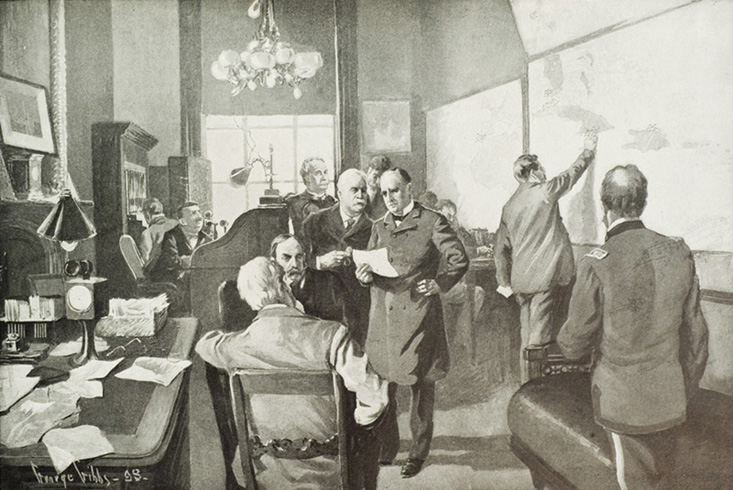
\includegraphics[width=13em]{warroom.jpg}}
	\end{columns}
\end{frame}
%--- Next Frame ---%

% section extensiveForm (end)


\end{document}